\documentclass[a4paper,11pt]{article}
\usepackage[dvipdfmx]{graphicx}
\usepackage{here}
\begin{document}

\title{Smartcab}
\author{Ryosuke Honda}
\date{2016/06/23}

\maketitle

\section{Implement a basic driving agent}
Implement the basic driving agent, which processes the following inputs at each time step:
\begin{itemize}
\item Next waypoint location, relative to its current location and heading.
\item Intersection state(traffic light and presence of cars) and
\item Current deadline value(time steps remining)
\end{itemize}
And produces some random move/action [None,'forward','left','right']
\section{Identify and update state}

\section{Implement Q-learning}
One of the most important breakthroughs in reinforcement learning was the development of Q-learning.Its simplest form,one step Q-learning, is defined by

\begin{equation}
	Q(s,a)\leftarrow (1-\alpha)Q(s,a)+\alpha(r(s,a)+\gamma \max_{a'}(Q'(s',a')))
\end{equation}
$\alpha$:Learning rate \\
$\gamma$:Discount rate \\
{\bf s} stands for state, {\bf a} stands for action, {\bf s'} stands for the next state, {\bf a'} stands for the all actions


First, set the parameters($\alpha$,$\gamma$) and environmental reward.Then Initialize the Q table to zero. For each episode, select a random initial state and do the following things until the agent has reached the goal.
\begin{itemize}
\item Select one among all possible actions for the current state.
\item Using this possible action, consider going to the next state.
\item Get maximum Q value for this next state based on all possible actions
\item Compute Q value
\item Set the next state as the current state
\end{itemize}


The Gamma and Alpha parameters has a range of 0 to 1. If Gamma is closer to zero, the agent will tend to consider only immediate rewards. If Alpha is closer to zero, the agent will tend to consider only past experience(don't learn).

The reward and penalty for this task is as follows.

\section{Enhance the driving agent}

Report what changes you make to your basic implementation of Q-learning to achieve the final version of the agent.How well does it perform?
\\
When the agent just started, it has no q-value since the q-table is set to be 0. Therefore, at first I need to set the move randomly($\epsilon$-greedy).
With the probability of $\epsilon$, the agent moves randomly. This prevents the agent from falling into the wrong choice. 



%%Explanation for the First implementation
First, I implemented random action.The agent just moves random action("None","Forward","Left","Right") and doesn't learn anything from experience.
\\
In the agent.py file, I set $\epsilon$ to be 1(The agents moves randomly).
I define "Success Rate" to see the agent's performance.

[Success Rate]=[No.trials achieve goal before deadline]/[No. trials]
\\For these trials, the number of trials are 100.

In this experiment,I set the conditions as follows.


Success rate in this trial is 0.20.


\begin{figure}[H]
\begin{center}
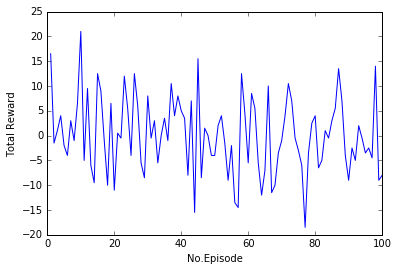
\includegraphics[width=100mm]{graph/random.jpg}
\end{center}
\caption{Random Action}
\label{fig:one}
\end{figure}

As the Fig\ref{fig:one} shows,the total rewards with this trial contains negative values.
Without learning from their experience, the agent won't get high reward.


%%Explanation for the Second Implementation

Second, the parameters of $\alpha$ and $\gamma$ are 0.5 and 0.9 respectively.
With this condition, the success rate is 0.72 which is higher than the random action.

\begin{figure}[H]
\begin{center}
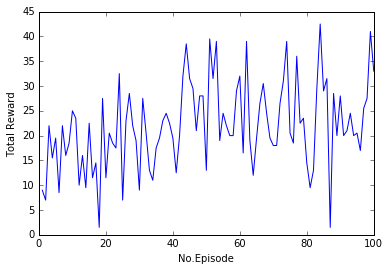
\includegraphics[width=100mm]{graph/constant.jpg}
\end{center}
\caption{Constant $\alpha$ and $\gamma$}
\label{fig:two}
\end{figure}

The Fig\ref{fig:two} shows,the total rewards for each episode are all positive and the cumulative sum of total reward of all episodes are 2195.5.




%%Explanation for the Third Implementation
Third, the parameters of $\alpha$ and $\gamma$ are as follows.

\begin{equation}
	\alpha=\frac{1.0}{1.0+time}
\end{equation}

\begin{equation}
	\gamma=\frac{1.0}{1.0+deadline}
\end{equation}

With this condition, the success rate is 0.86 which is higher than the trials before and the cumulative sum of total reward of all episodes are 2099.0


\begin{figure}[H]
\begin{center}
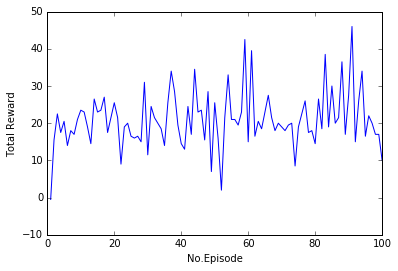
\includegraphics[width=100mm]{graph/better.jpg}
\end{center}
\caption{Fig}
\label{fig:three}
\end{figure}

The condition in this agent is


%%Explanation for the Final Implementation
Final version

\begin{figure}[H]
\begin{center}
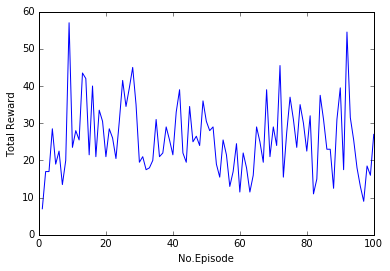
\includegraphics[width=100mm]{graph/gamma_con.jpg}
\end{center}
\caption{Fig}
\label{fig:three}
\end{figure}

\end{document}